\documentclass{amsart}

%     If your article includes graphics, uncomment this command.
\usepackage{graphicx}
\usepackage{amsmath,amsfonts,amssymb,amscd,amsthm,amsbsy,upref}
\usepackage[all]{xy}
\usepackage{amsmath}
\usepackage{mathrsfs}
\usepackage{paralist}
\usepackage{setspace}
\usepackage{graphicx}
\usepackage{tikz-cd}
\usepackage{pgfplots}
\usepackage{fancyhdr}
\usepackage{tikz}
\usepackage{pgfplots}
\usepackage{array}
\usepackage{listings}
\setlength{\textwidth}{\paperwidth}
\addtolength{\textwidth}{-3in}
\calclayout

\newtheorem{theorem}{Theorem}[section]
\newtheorem{lemma}[theorem]{Lemma}

\theoremstyle{definition}
\newtheorem{definition}[theorem]{Definition}
\newtheorem{example}[theorem]{Example}
\newtheorem{xca}[theorem]{Exercise}

\theoremstyle{remark}
\newtheorem{remark}[theorem]{Remark}

\numberwithin{equation}{section}

%    Absolute value notation
\newcommand{\abs}[1]{\lvert#1\rvert}

%    Blank box placeholder for figures (to avoid requiring any
%    particular graphics capabilities for printing this document).
\newcommand{\blankbox}[2]{%
  \parbox{\columnwidth}{\centering
%    Set fboxsep to 0 so that the actual size of the box will match the
%    given measurements more closely.
    \setlength{\fboxsep}{0pt}%
    \fbox{\raisebox{0pt}[#2]{\hspace{#1}}}%
  }%
}

\begin{document}

\title{Assigning Scouts to Optimal Patrols}
\author{Phil Snyder}
\author{Ian Bruce}
\author{Julio Marco Pineda}

\begin{abstract}
Scoutmaster Gene Bruce of the Boy Scouts of America for Troop 407 in Kent, Washington wants to find an arrangement of 13 new scouts into two patrols. The cohesiveness and overall quality experience of a patrol is affected by conflicting relationships and existing friendships. If enough adverse encounters occur in one patrol, the scouts may decide to drop out from the organization all together, missing out on a potentially great experience and community of friends. Thus our project focuses on helping the Scoutmaster find an optimal arrangement of the new scouts into tw patrols By using anonymous data from scouts and parents, a brute force strategy was employed to find an optimal arrangement of scouts that avoids severe conflict while maximizing pre-existing preferences. 
\end{abstract}

\maketitle
\section*{Problem Description}
The community partner we are serving for this project is Scoutmaster Gene Bruce of the Boys Scouts of America. He leads Troop 407 in Kent, Washington and every year he must assign new scouts to groups - called ``patrols''. In these patrols, scouts perform different scouting activities together and form close bonds. However, in recent years, the number of scouts have been increasing at such a rate that it is no longer logistically viable to place every new scout in a single patrol; multiple patrols are needed to organize activities better and to form a community between new recruits. Furthermore, scouts are in the fifth or sixth grade and have not yet fully developed their interpersonal skills. Many can be temperamental and awkward when dealing with adversity. Devastating conflicts may occur if two at-odds scouts create animosity between each other, alienating themselves from the rest of the patrol. If enough of these adverse interactions occur within a patrol, scouts may decide to drop out of the Boy Scouts, losing out on a potentially great experience and community of friends.

The data the Scoutmaster collects about adverse pairings and preferences are either privately given by the scouts themselves or by their parents. The parents preferences are hard rules that we must abide by (if possible). In the past, the Scoutmaster determined the perfect arrangement of patrols without too much time and effort due to the smaller number of new recruits. However, newer scouts are joining yearly to the point that solving this grouping problem cannot be done by hand in a reasonable amount of time. Therefore, we can help our community partner find a better means to solve his troop organization problem. Our goal is to assign boy scouts in different patrols of appropriate size (of 6-8 scouts) such that we maximize the retention rate of the scouts in the program by avoiding severe conflicts while maximizing positive relationships between scouts.

We aim to answer the particular instance of this problem provided by our community partner, that of arranging 13 scouts into two troops that avoids severe conflicts while promoting positive relationships between scouts. Furthermore, we want to determine if we can build a model to determine optimal patrol arrangements for any number of scouts so that the Scoutmaster can use this model for future years. For 13 scouts, a grouping into one patrol is too large, while three patrols are too small, and need not be considered. But in general it is possible to calculate all possible partitions with size constraints on the partitions for an arbitrary number of scouts\cite{B}. 

Furthermore, this model can be applied to other situations where interpersonal dynamics is important. For example, elementary school students usually are arranged into groups during class activities. The kids that formed supportive groups tend to have more enthusiastic students, enhancing their enjoyment and learning during the lesson \cite{D}. Another example is military personnel that conduct missions in troops. The harmony and cooperation within a troop is necessary to form trust for the success of their mission and, at times, survival of the entire group \cite{E}. 

The 13 different recruited scouts are Brandon, Cameron, Christian, Colby, Daniel, Darwin, Evan, Jake, Jordan, Nathan, Patrick, Timmy and Tommy. After the Scoutmaster collected the likes and dislikes of each scout, he presented the data as follows: 
\begin{figure}[h]
	\centering
	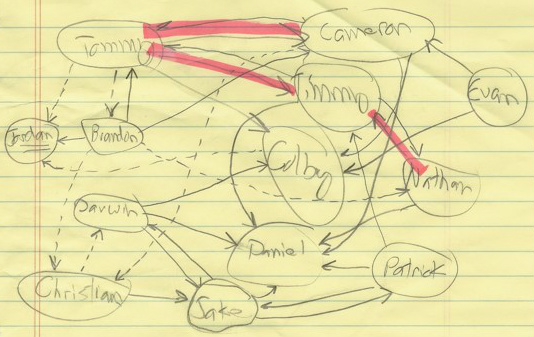
\includegraphics[scale=0.60]{graph}
\end{figure}

The solid arrow represents a preferred companion. For example, there is a solid arrow from Tommy pointing to Colby indicating that Tommy likes to be with Colby. A dashed arrow represents a dislike. For example, there is a dashed arrow from Tommy to Jordan showing that Tommy does not want to be with Jordan. Furthermore, the Scoutmaster provided us a separate email, and indicated that Colby and Jordan cannot be in the same troop (as per a parental request). The highlighted arrows in the figure indicate a mutual friendship between scouts.

The Stirling number of the second kind provides the total possible ways to arrange any number of distinguishable objects to indistinguishable groups as long as any troop size is permitted (except the empty troop) \cite{F}. For the data in this project, the Stirling number of the second kind for 13 scouts into 2 troops is 4095 (see \textit{Appendix B}). This number provides an upper bound on the possible arrangements for the specific problem tackled in this project.

\section*{Simplifications}
Ultimately, our goal is to find groups for the scouts that will allow them to enjoy their time scouting to the fullest. Modeling interpersonal relations by likes and dislikes is, of course, a simplification. But the difficulty in modeling the intricacies of human relationships demands it. In addition, our process will have to be repeated each year for every new batch of scouts, and would perhaps be too burdensome to warrant the effort if our process attempted to delve too far into the psyche.

Another simplification is to assume that the quality of a group can be determined by the quality of relationships between unique pairs either inside or outside the group - in other words, the whole is equal to the sum of the parts. For example, consider the case where scouts A, B and C individually like each other when they are alone with one of their group, but do not like being in a group together. This type of epiphenomenon will not be considered.

\section*{Mathematical Model}
To model the relationships between scouts, we use a mathematical graph. A graph is a convenient way to illustrate direct relationships between pairs of objects; and a good example that explains how they work is to consider roads between cities. On a map, we consider two cities to be ``connected" if they share a road between them; by this, we mean that the existence of a road defines the property of two cities being connected. Graphs abstract this notion; instead of considering connections between a map of cities, we consider connections between groups of any kind of object. In graph theoretic terminology, we call these objects vertices, and the entity that connects two vertices is called an edge. We could redefine our map of cities in this terminology: consider cities as being vertices in a graph where the criterion for having an edge between two vertices is when there is a road built between the cities. Another common optional property of graphs is where we ascribe numbers to the edges, corresponding to particular ``weights" that they have. In our city graph example, we could consider each edge to have a weight of how long the road is. Edges can even be directed, meaning that a particular relationship between vertices is only valid from one vertex to another, and not the other way around. For example, there could be a one-way road from city A to city B, and no road from city B to city A. In our situation, we will also consider graphs that are complete, where completeness means that each vertex is connected to every other vertex.

For our problem, we can define a graph where scouts are vertices. A directed edge between Scout A and Scout B has a weight proportional to how much Scout A likes Scout B. We give the directed edge between scout A and scout B a weighting of 1 if A likes B, 0 if A is indifferent to B, and a -1 if A disapproves of B. This results in a complete, directed graph of 13 vertices, since there are 13 scouts. Note that these edges are directed; we want to consider cases where the relationship between two scouts is not symmetric, whereas a weighted undirected graph would not be able to represent this asymmetry. Let us now define a $k$-partition of a graph as a grouping of vertices where each vertex is assigned into one of $k$ groups where $k$ is a natural number; thus, a $k$-partition of the vertices in the scout graph would represent splitting up the scouts into $k$ different patrols. Scoutmaster Bruce specifically would like two patrols from the 13 scouts - one of size 6, the other of size 7, which means that we need to find a 2-partition of the graph where 6 vertices are in one grouping and 7 are in the other. The total number of partitions given these constraints is $\binom{13}{6} = \binom{13}{7} = 1716$. Given these 1716 partitions, we want to select one of them that is ``best" for the scouts in question. In mathematics, picking the ``best" option out of a list of options corresponds to first defining a function that ``scores" how good an item is (or bad an item is) and then picking the item with the highest score (or the least score, if our scoring function defines how bad an item is). This process of selecting the item from a list that has the most extreme score is called optimization. From now on, we will call these scoring functions objective functions. Our process for optimizing a partition of the scouts will become computing an objective function for each possible partition and then selecting the partition that gives us the most extreme score. This ``brute force" approach to computing the scores isn't always appropriate for optimizing an objective function over a set of values, as the size of the set of values is too large for a computer to iterate over in a timely fashion. Often, a more sophisticated technique will be required to iterate over a manageable subset of the set of possible values. However, 1716 is within the range of sizes of sets to iterate over where we could apply a brute force technique to solve for the most optimal partition.

We provide six different objective functions that we deemed reasonable for measuring how well patrol partitions would work. We dub each of these functions MinCut, FriendCut, EnemyCut, AwkwardCut (+1), AwkwardCut (+2), and HybridCut. MinCut is designed to minimize the cut edge weights between partitions (see \textit{Solution of Mathematical Problem}). FriendCut is designed to maximize the number of intra-patrol positive edge weights. EnemyCut is meant to minimize the number of intra-patrol negative edge weights, Awkward cut ($+i$) is the same as MinCut, but with an additional penalty of $i$ if there are a pair of scouts, Scout A and Scout B, such that Scout A favors Scout B, but Scout B disfavors Scout A. HybridCut is a convex combination of MinCut and FriendCut, each with equal weight (that is, half the MinCut loss plus half the FriendCut loss). Our three primary objective functions - MinCut, FriendCut, and EnemyCut are given a more rigorous treatment in the next section.

\section*{Solution of Mathematical Problem}
We represent our directed graph as a 13 by 13 similarity matrix, or, as might
be more fitting for the problem, an ``affinity'' matrix. Like below\footnote{The scouts were enumerated like so: 1. Brandon, 2. Cameron, 3, Christian, 4. Colby, 5. Daniel, 6. Darwin, 7. Evan, 8. Jake, 9. Jordan, 10. Nathan, 11. Patrick, 12. Timmy, 13. Tommy.}:

\begin{figure}[h]
    \centering
    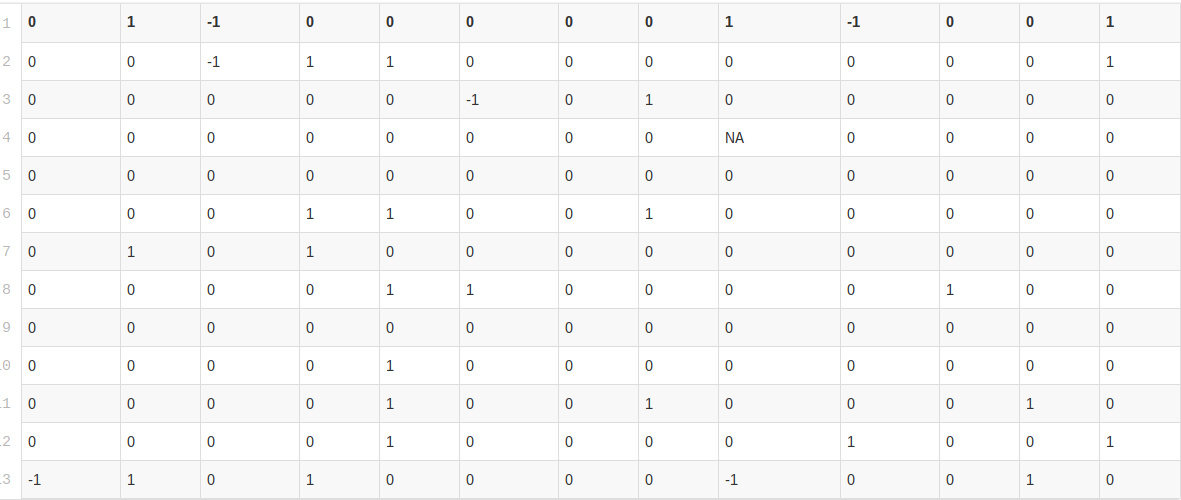
\includegraphics[scale=0.28]{data}
\end{figure}
%%%%%%%%%%%%%%%%%%%%%%%%%%%%%%%%%%%%%%%%%%%%%%%%%%%%%%%%%%%%%%%%%%%%%%%%
%%%%%%%%%%%%%%%%%%%%%%%%%%%%%%%%%%%%%%%%%%%%%%%%%%%%%%%%%%%%%%%%%%%%%%%%

The NA value represents a hard constraint established by a scout's parent (i.e., under no circumstances are these two to be in the same patrol). We designed a number of objective functions that accept two scouts and calculates the loss associated with such a placement.

\section*{Results}
As mentioned earlier, the number of scouts we must partition is small enough to find an optimal solution by brute force. Our algorithm finds a partition of scouts into patrols of sizes 6 and 7 which is optimal with respect to each objective.

\begin{figure}[h]
\centering
\begin{tabular}{ |l|l|l|l|l|l| }
\hline
\multicolumn{2}{|c|}{\textbf{MinCut}} & \multicolumn{2}{|c|}{\textbf{FriendCut}} & \multicolumn{2}{|c|}{\textbf{EnemyCut}}\\
\hline
Patrol 1 & Patrol 2 & Patrol 1 & Patrol 2 & Patrol 1 & Patrol 2\\
\hline
Brandon & Christian & Brandon & Daniel & Brandon & Christian\\
Cameron & Daniel & Cameron & Darwin & Cameron & Jake\\
Colby & Jake & Christian & Jake & Colby & Jordan\\
Darwin & Jordan & Colby & Jordan  & Daniel & Nathan\\
Evan & Nathan & Evan & Nathan & Darwin & Patrick\\
Tommy & Patrick & Tommy & Patrick & Evan & Timmy\\
& Timmy & & Timmy & Tommy & \\
\hline
\multicolumn{6}{|c|}{\hphantom{1}} \\
\hline
\multicolumn{2}{|c|}{\textbf{AwkwardCut (+1)}} & \multicolumn{2}{|c|}{\textbf{AwkwardCut (+2)}} & \multicolumn{2}{|c|}{\textbf{HybridCut}} \\
\hline
Patrol 1 & Patrol 2 & Patrol 1 & Patrol 2 & Patrol 1 & Patrol 2\\
\hline
Brandon & Christian & Brandon & Cameron & Brandon & Christian\\
Cameron & Daniel & Christian & Evan & Cameron & Daniel\\
Colby & Jake & Daniel & Colby & Colby & Darwin\\
Darwin & Jordan & Darwin & Nathan & Evan & Jake\\
Evan & Nathan & Jake & Timmy & Timmy & Jordan\\
Tommy & Patrick & Jordan & Tommy & Tommy & Nathan\\
\hphantom{1} & Timmy & Patrick & \hphantom{1} & \hphantom{1} & Patrick\\
\hline
\end{tabular}
\caption{The partitions arrived at by minimizing each objective function}
\end{figure}

For each method we define three scoring metrics:

\begin{enumerate}
\item \textbf{MinCut}. This is the traditional metric of a cut on a weighted graph and is the sum of the weights of the edges we would ``cut'' if we were to sever the edges between distinct patrols. More formally, for some partition $I, J$ $I \neq J$, the MinCut is defined as:
$$
MinCut(I, J) := \sum_{e = (i, j), i \in I, j \in J}^{} c(e)
$$
We want this to be as low as possible.
\item \textbf{FriendCut}. This is the sum of the positive, or friendly edge weights within each patrol. That is, if $I_+ = \{e=(i,j) | i,j \in I, c(e)=1\}$ is the the set of edges in patrol $I$ with positive weight and $J_+ = \{e=(i,j) | i,j \in J, c(e)=1\}$ is the set of edges in patrol $J$ with positive weight, then (assuming all positive weights are 1):
$$
FriendCut(I, J) :=  |I_+ \cup J_+|
$$
We want this to be as high as possible.
\item \textbf{EnemyCut}. This is similar to FriendCut, except we now measure the number of negative edges going from one scout to another within the same patrol. Let $I_- = \{e=(i,j) | i,j \in I, c(e)=-1\}$ be the the set of edges in patrol $I$ with negative weight and $J_- = \{e=(i,j) | i,j \in J, c(e)=-1\}$ be the set of edges in patrol $J$ with negative weight, then
$$
EnemyCut(I, J) := |I_- \cup J_-|
$$
    We want this to be as low as possible.
\end{enumerate}

The other methods are modifications of these three and are defined in Appendix A.

\begin{figure}[h]
    \centering
    \begin{tabular}{ |l|l|l|l| }
        \hline
        \textbf{Method} & \textbf{MinCut} & \textbf{FriendCut} & \textbf{EnemyCut} \\
        \hline
        MinCut & 0 & 17 & 0 \\
        FriendCut & 1 & 18 & 1 \\
        EnemyCut & 2 & 15 & 0 \\
        AwkwardCut (+1) & 0 & 17 & 0 \\
        AwkwardCut (+2) & 1 & 18 & 2 \\
        HybridCut & 0 & 18 & 1 \\
        \hline
    \end{tabular}
    \caption{The scores according to the three primary metrics.}
\end{figure}

Of the objective functions we chose to use, it seems as though MinCut and HybridCut are the best performing. FriendCut performs almost as well as HybridCut, except for one worse in the EnemyCut objective. EnemyCut does poorly since finding a partition with 0 intra-patrol negative weight edges is easy in this example, and so EnemyCut settles for the first suboptimal (in terms of the other objective functions) solution it finds. AwkwardCut (+1) arrived at the same partition as MinCut (not altogether surprising, but informative, since even with the additional +1 penalty for placing Brandon and Tommy in the same patrol it decided it would be best off to do so anyways). But changing the ``awkward'' penalty to +2, the same penalty as mutual dislike in EnemyCut, we get a completely different partition.

Let us take a more critical look at the optimal partition arrived at via MinCut:

\begin{table}[h]
	\caption{The partition arrived at by optimizing MinCut}\label{eqtable}
	\renewcommand\arraystretch{1.5}
	\noindent\[
	\begin{array}{|c|c|}
	\hline
	\textbf{Patrol 1}&\textbf{Patrol 2}\\
	\hline
	\text{Brandon, Cameron, Colby,}&\text{Christian, Daniel, Jake,}\\
	\text{Darwin, Evan, Tommy}&\text{Jordan, Nathan, Patrick, Timmy}\\
	\hline
	\end{array}
	\]
\end{table}

\begin{enumerate}
	\item Tommy and Timmy both like each other and are in separate patrols. But if we move Timmy to Patrol 1 ($P1$), we break up the mutual friendship of Timmy and Nathan in $P2$. Suppose we moved both Timmy and Nathan to $P1$ and Brandon (who dislikes Nathan) to $P2$. But then Brandon loses two friends (Tommy and Cameron), gains one (Jordan), and now neither Nathan nor Timmy are in the same patrol as Daniel, whom they both like. Although, Brandon and Tommy find themselves in the awkward situation of having complete opposite sentiments towards each other. Perhaps this would be a worthwhile trade after all (and a larger, negative weight needs to be placed upon disfavor-favor relationships).
	
	\item As mentioned in the previous point, Tommy dislikes Brandon. Trading Tommy in $P1$ for Jordan in $P2$ seems promising, but we have overlooked the fact that Colby and Jordan are our NA pair, and cannot be in the same patrol under any circumstances. Trading Colby for Jordan is another option, but Colby will be missed by Darwin, Evan, Cameron and Tommy (In other words, the whole of P1 minus Brandon).
\end{enumerate}

On the whole, though, there are no obvious improvements that can be made to our algorithm's partitions. We find that this is an assignment that could have reasonably been arrived at by Scoutmaster Bruce (granted the group dynamics have not changed since the scouts were surveyed).  Furthermore, the solution took only 10 seconds to arrive at on a single core machine.

\section*{Improvements}
While our algorithm demonstrably works well on smaller groups of 13 people, we do not expect our brute force solution to be tractable on larger groups wherein greater than 2 partitions are required. As a possible scenario, consider a company of 150 people to be divided into fixed-size teams of 10 individuals each. There are $150! / (10!)^{15}$ possible partitions, a number proportional to $10^{164}$ - meaning we could instead use that computational time to enumerate the number of atoms in the universe\ldots a tredecillion $(10^{78})$ times. Knowing this, perhaps it will not surprise the reader that this particular graph partitioning problem in general graphs is NP-complete - though there do exist approximation algorithms \cite{A}.
As scout enrollment increases, it becomes necessary to consider scenarios where we have both a large number of scouts in need of assignment and multiple patrols to choose from. Our algorithm could be extended to use brute force to find a globally optimal solution when it is deemed computationally feasible and to use an approximating algorithm to find a locally optimal solution otherwise. 

\section*{Conclusions}
Assigning individuals to compatible groups is hard (computationally speaking). When the group is small enough - as it is here - globally optimal solutions may be arrived at by checking all feasible solutions. However, the amount of computation time needed to arrive at an answer grows exponentially with the number of individuals and groups. For example, finding an optimal partition of 13 scouts into \textit{three} groups would take over 50 times as long as finding the optimal partition of 13 scouts into two groups (90,090 feasible combinations to check versus 1,716 in the two patrol case).


Nevertheless, our chosen objective functions seem to arrive at solutions that are able to hold up to human scrutiny, and perform well enough when total enumeration is possible. Larger problems may require approximating or clustering methods\footnote{Hartigan, J. A., and M. A. Wong. "Algorithm AS 136: A K-Means Clustering Algorithm." Applied Statistics 28.1 (1979): 100.}. 

\section*{Acknowledgments}
We would like to thank Scoutmaster Gene Bruce for his cordiality and for providing us the necessary data. We would also like to thank Professor Sara Billey for her mentorship and guidance provided throughout our project. 

\section*{Verification Statement}
Scoutmaster Gene Bruce addressed our professor, Sara Billey, with the following comments: ``I'd like to thank you and your students for developing a process to divide a group of new scouts into patrols based upon solicited personal preferences.  While a relatively small problem, it can take a lot of effort to solve by hand.  The students grasped the subtleties of the conflicting objectives.  I appreciated their approach of using multiple objective functions.  This provided a family of solutions that gave insights into the problem.  I appreciate this much more than a process that produces the ``one best answer".  It's much easier for me to add my ``gut instinct" with a handful of alternatives rather than the original 1716 possible combinations.  I look forward to setting up the process on my home computer and leveraging it during the next recruiting season."
\section*{Appendix A}
The other objective functions.

\begin{enumerate}
    \item \textbf{AwkwardCut (+i)}. Same in all respects to MinCut, except for an additional penalty of $i$ if there are two scouts, Scout A and Scout B, in the same patrol such that Scout A likes Scout B and Scout B dislikes Scout A.
    \begin{equation*}
        \begin{split}
            AwkwardCut&(I, J, i) := \Bigg[ \sum_{e = (k, j), k \in I, j \in J}^{} c(e) \Bigg] \\
            &+ i * \left\vert{\{e_+ = (k,j), e_- = (j, k) : e_+, e_- \in I, c(e_+) = 1, c(e_-) = -1\}}\right\vert
        \end{split}
    \end{equation*}

\item \textbf{HybridCut}. A convex combination of MinCut and FriendCut, each with equal weight (that is, half the MinCut loss plus half the FriendCut loss).
    \begin{equation*}
        HybridCut(I, J) := \frac{1}{2}MinCut(I, J) + \frac{1}{2}FriendCut(I, J)
    \end{equation*}
\end{enumerate}

\section*{Appendix B}
The solution for finding the Stirling number of the second kind for $n = 13$ scouts to be arranged in $k = 2$ troops:
\begin{gather*}
	S(n,k) = \frac{1}{k!} \sum_{i=0}^{k}(-1)^k {2 \choose i} (k - i)^{n} \\
	S(13,2) = \frac{1}{2!} \sum_{i=0}^{2}(-1)^2 {2 \choose i} (2 - i)^{13} \\
	S(13, 2) = 4095
\end{gather*}

\clearpage

\section*{Appendix C}
Scoutmaster Gene Bruce wanted to arrange 13 scouts into two groups where one group will have 6 scouts and the other will have 7 scouts. We can find the number of combinations possible of the 13 scouts into a troop size of 6 or 7 using the binomial coefficient.

Let us first tackle a simpler problem to understand how to find the number of combinations. Suppose we have 4 people: A, B, C and D that we want to form groups of size 3 where the order of people does not matter. The possible combinations are:

\begin{itemize}
	\item A,B,C	
	\item A,B,D
	\item A,C,D	
	\item B,C,D
\end{itemize}
Thus, there are 4 different combinations of grouping 4 people in a group of size 3. It would be impractical to list out all the possible combinations for larger number of people, thus we use the binomial coefficient formula \cite{F}:
\begin{gather*}
	\binom{n}{r} = \frac{n!}{r!(n-r)!}
\end{gather*}
where $n$ is the number of people and $r$ is the size of the group. For this small problem:
\begin{gather*}
	\binom{4}{3} = \frac{4!}{3!(4-3)!} = \frac{4\cdot3!}{3!1!} = 4
\end{gather*} 
Thus, we can see we arrive with the same result.

Now to address the question of arranging 13 scouts into a troop of size 6:
\begin{gather*}
	\binom{13}{6} = \frac{13!}{6!(13-6)!} = 13!/(6!7!) = 1716
\end{gather*}
The other troop would have a size of 7:
\begin{gather*}
	\binom{13}{7} = \frac{13!}{7!(13-7)!} = 13!/(7!6!) = 1716
\end{gather*}
Therefore the number of combinations possible for arranging 13 scouts into 6 or 7 troop size is 1716.
\bibliographystyle{amsplain}
\begin{thebibliography}{10}

\bibitem {A} B. W. Kernighan, S. Lin, \textit{An Efficient Heuristic Procedure for Partitioning Graphs}. Bell System Technical Journal. \textbf{49} (1970), 291--307. doi: 10.1002/j.1538-7305.1970.tb01770.x

\bibitem {B} Desquelles, P. ``Calculation of the Number of Partitions with Constraints on the Fragment Size." Phys. Rev. C Physical Review C 65.3 (2002)

\bibitem {C} Hartigan, J. A., and M. A. Wong. "Algorithm AS 136: A K-Means Clustering Algorithm." Applied Statistics 28.1 (1979): 100.

\bibitem {D} Mendoza, Veronica, ``Mabel Paine Elementary School classroom helper." \textit{Personal Communication}.

\bibitem {E} Lin, Kevin. ``Air Force ROTC Cadet in the 910th Cadet Wing." \textit{Personal Communication}.

\bibitem {F} Roberts, F., Tesman, B. ``Applied Combinatorics Second Edition." \textit{CRC Press}. 2009. Pp 54-55.

\clearpage

\section*{Code}

\begin{lstlisting}
from __future__ import print_function
import pandas as pd
import numpy as np
import matplotlib.pyplot as plt
import itertools

data = pd.read_csv("data.csv", header=None, dtype='float')
data = data.fillna(float('-inf'))
names = pd.read_csv("names.csv", header=None)

'''
Traditional Min Graph Cut

Change in loss function for scouts in *different* patrols

mutual friends: +2
one like, one indifferent: +1
one like, one dislike: 0
one dislike, one indifferent: -1 
mutual enmity: -2
'''
def min_cut(pair, in_same_patrol):
	x, y = pair
	if not in_same_patrol:
		return max(-2, data[x][y] + data[y][x])
	else:
		return 0

'''
Friendly Cut: maximize friendship within patrol

Change in loss function for scouts in *same* patrol:

mutual friends: -2
one like, one indifferent: -1
one like, one dislike: 0
one dislike, one indifferent: 0 
mutual enmity: 0
'''
def friendly_cut(pair, in_same_patrol):
	x, y = pair
	if in_same_patrol:
		return -1 * max(0, data[x][y] + data[y][x])
	else:
		return 0

'''
Enemy Cut: minimize enemies within patrol

Change in loss function for scouts in *same* patrol:

mutual friends:0 
one like, one indifferent: 0
one like, one dislike: 0
one dislike, one indifferent: +1 
mutual enmity: +2 
'''
def enemy_cut(pair, in_same_patrol):
	x, y = pair
	if in_same_patrol:
		return max(0, -(data[x][y] + data[y][x]))
	else:
		return 0

'''
Awkward Cut: same as Min Cut but with additional penalty
for one like, one dislike in same patrol

Change in loss function:

mutual friends: +2
one like, one indifferent: +1
one like, one dislike (same patrol): +1
one like, one dislike (different patrol): 0
one dislike, one indifferent: -1 
mutual enmity: -2
'''
def awkward_cut(pair, in_same_patrol):
	x, y = pair
	if in_same_patrol and data[x][y] == -data[y][x] and abs(data[x][y]) > 0:
		return 1 
	elif not in_same_patrol:
		return max(-2, data[x][y] + data[y][x])
	else:
		return 0

def hybrid_cut(pair, in_same_patrol):
	return 0.5 * min_cut(pair, in_same_patrol) \
		+ 0.5 * friendly_cut(pair, in_same_patrol)

# this function assumes that the partitions are disjoint, no
# check for this has been implemented
def calculate_loss(partition, objective):
	def compare_pair(pair): # returns true if pair is in the same partition,
		ans = False         # false otherwise
		for part in partition:
			ans = ans or (pair[0] in part and pair[1] in part)
		return ans
	total = ()			# total will include every element in the
	loss = 0			# partitions
	for part in partition:
		total += tuple(part)
	every_pair = itertools.combinations(total, 2)
	for pair in every_pair:
		loss += objective(pair, compare_pair(pair))
	return loss

def brute_force_solver(d=data, num_patrols=2, objective=min_cut, min_patrol_size=6, max_patrol_size=7):
	partitions = generate_partitions([], num_patrols, len(d))
	best_partition_so_far = None
	best_loss = float('inf')
	for part in partitions:
		if (sum(part) >= min_patrol_size and sum(part) <= max_patrol_size \
			and not (part[3] and part[8]) and not(not(part[3] or part[8]))):
			if any([3 in p and 8 in p for p in partitions]): print('hello')
			patrols = [[] for i in range(num_patrols)]
			for i in range(len(part)):
				patrols[part[i]] += [i]
			loss = calculate_loss(patrols, objective)	
			if loss < best_loss:
				best_partition_so_far = patrols
				best_loss = loss
	return best_partition_so_far, best_loss

def generate_partitions(arr, patrols, num_scouts):
	result = []
	if num_scouts == 0:
		return [arr]
	else:
		for i in range(patrols):
			for c in generate_partitions(arr + [i], patrols, num_scouts - 1):
				result += [c]
	return result
'''
Example use

best_patrol, best_loss = brute_force_solver()
print "Best patrol:", best_patrol
print "Loss:", best_loss
'''
\end{lstlisting}
\end{thebibliography}

\end{document}

%------------------------------------------------------------------------------
% End of journal.tex
%------------------------------------------------------------------------------
